% !TEX encoding = UTF-8 Unicode
%Präambel

%Report für große Doukumente. Dieser ist in Kapitel (\chapter{}) aufgeteilt
%\documentclass[12pt, a4paper, ngerman]{report} 

%Article für normale Doumente
\documentclass[12pt, a4paper, ngerman]{article}

%Deutsche Beschreibungen von generiertem Text (table of contents => Inhaltsverzeichnis)
\usepackage[ngerman]{babel}

%Umlaute
\usepackage[utf8]{inputenc}

%Schriftart Helvetica 
\usepackage[scaled]{helvet}

%Seitenränder
\usepackage{geometry}
%top = Abstand nach oben
%left = Abstand nach links
%right = Abstand nach rechts
%bottom= Abstand nach unten
%heapsep= Abstand zwische Kopfzeile und Text
%footskip= Abstand zwischen Text und Fußzeile
\geometry{a4paper, top=25mm, left=30mm, right=25mm, bottom=30mm, headsep=10mm, footskip=12mm}

%Farben nutzen
\usepackage{xcolor}

%Grafiken einbinden
\usepackage{graphicx}

%Zusätzliche Positionsbefehle
\usepackage{float} 

%Die Einrücktiefe bei einem neuen Absatz
\setlength{\parindent}{0pt}


%Fülltext
\usepackage{blindtext}

%Fuer Zitate	
\PassOptionsToPackage{backend=bibtex}{biblatex}
\usepackage[natbib=true,style=numeric]{biblatex}
\usepackage[babel,german=guillemets]{csquotes}
\bibliography{quellen.bib} 


%Eigene Kommandos
% Osi Modell
\newcommand{\osi}{ISO/OSI Referenzmodell\xspace}

%Ende Präambel
	
\begin{document}

\begin{titlepage}
		\begin{center}
			
\includegraphics[width=.8\linewidth]{Grafiken/logo_htw.jpg}\\[1cm]    
			\textsc{\LARGE Hochschule für Technik und Wirtschaft \newline Fakultät für Ingenieurwissenschaften}\\[1.5cm]
			\newcommand{\HRule}{\rule{\linewidth}{0.5mm}} \HRule \\[0.4cm] { \huge \bfseries Ausarbeitung Protokolle}\\[0.4cm]
			\HRule \\[1.5cm]

			\begin{minipage}{0.4\textwidth}
				\begin{flushleft} \large
					\emph{Autoren:}\\
					Deniz \\
					Christoph Drost 3576450
				\end{flushleft}
			\end{minipage}
			\hfill
			\begin{minipage}{0.4\textwidth}
				\begin{flushright} \large
					\emph{Betreuer:} \\
					Jonas Vogt, M.Sc.
				\end{flushright}
			\end{minipage}
			\vfill
			{\large \today}
		\end{center}
	\end{titlepage}


%Inhaltsverzeichnis auf eigener Seite
\tableofcontents
\newpage 

\section{Einleitung}
Im Folgenden sollen verschiedene Layer 2 Protokolle für kabelgebundene Netze miteinander verglichen werden. Um die Zusammenhänge besser erklären zu können, möchten wir erst auf das \osi eingehen.
\subsection{Das \osi}
\begin{figure}[h]
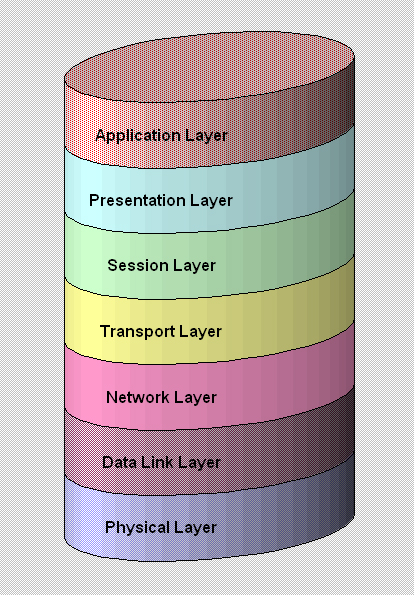
\includegraphics[width=0.5\textwidth]{Grafiken/osi_modell.jpg}
\caption{Das \osi im Überblick \cite{osi_modell}}
\label{osi_modell}
\end{figure} 
Diese Grafik stellt die Schichten des \osi da. Das \osi, (Open Systems Interconnection Model) ist ein allgemeines Kommunikationsmodell,  das die Kommunikation unterschiedlichster Geräte ermöglicht. Es beschreibt ein komplettes Telekommunikationsnetzwerk. Die einzelnen Funktionen sind in 7 Schichten aufgeteilt. 

Das \osi standardisiert die Netzwerk Architektur. Dadurch können Hersteller Lösungen anbieten, die auf der ganzen Welt genutzt werden können. Eine proprietäre Lösung hätte zu Insellösungen geführt. Ein weiterer Vorteil ist, dass die einzelnen Schichten, oder Layer, über Schnittstellen miteinander kommunizieren. Das ermöglicht ein Austauschen einzelner Komponenten, ohne die gesamte Architektur ändern zu müssen.

Da das \osi nur ein Referenzmodell darstellt, müssen die einzelnen Schichten konkret implementiert werden. Diese Implementierungen sind eigene Protokolle. 

\subsection{Der Layer 2}
Der Layer 2, Data Link Layer, setzt auf dem Physical Layer auf und stellt dem Network Layer seine Dienste zur Verfügung. Der Physical Layer beschriebt das Medium über das die Signale übertragen werden. Hier findet noch keine Logik statt. 

Die Aufgaben des Layer 2 im Überblick:
\begin{itemize}
	\item Aufteilung in Pakete
	\item Fehlerkontrolle
\end{itemize} 

\subsubsection{Aufteilung in Frames}
Die Datenblöcke werden im Layer 2 in Frames aufgeteilt. Die Vorteile des Framing sind die schnellere Nutzung eines shared Mediums und dass fehlerhafte Daten nicht komplett übertragen werden müssen.
\subsubsection{Fehlerkontrolle}
Der Data Link Layer führt eine Fehlerkontrolle durch. Dazu zählen eine Suche nach Duplikaten, nach inkorrekt oder unvollständig gesendeten Paketen. Wenn ein Fehler entdeckt wird, wird eine neue Übertragung der Frames angefordert \cite[S. 91]{SWB-107223570}. Die Fehlerkontrolle wird über den \glqq Cyclic Redundancy Check\grqq ~CRC durchgeführt. Dieses Verfahren ist eine Möglichkeit zur Prüfsummenberechnung, die beim Sender und der Senke durchgeführt wird. Sind beide Prüfsummen gleich, kann angenommen werden, dass das Frame korrekt übertragen wurde. 

Die Frames werden mit Sequence Numbers durchnummeriert. Der Empfänger prüft, ob die Frames in der richtigen Reihenfolge ankommen. Bei einer \glqq out-of-sequence transmission\grqq ~kann von einem verlorenen Frame ausgegangen werden, das entsprechende Frame wird neu angefordert.
\section{Die Layer 2 Protokolle im Überblick}

\subsection{Ethernet}
\blindtext

\subsection{LAPD}
\blindtext

\subsection{PPP}
Router - Router und Host - Netzwork Verbindungen über synchrone und asynchrone Kreise. Enthält ein Protokoll Feld um das Network Layer Protokoll zu Identifizieren \cite[S. 102]{SWB-107223570}  

\section{Bedeutungen der Protokolle im \osi }
%Quellenangabe auf eigener Seite
\newpage
\sloppy
\printbibliography 



%Abbildungsverzeichnis auf eigener Seite
\newpage
\listoffigures

\end{document}